A seguir, está descrito os passos para gerar um pacote de um jogo no Unity.

\begin{enumerate}
\item Acessar Edit > Project Settings > Player.

\begin{center}
	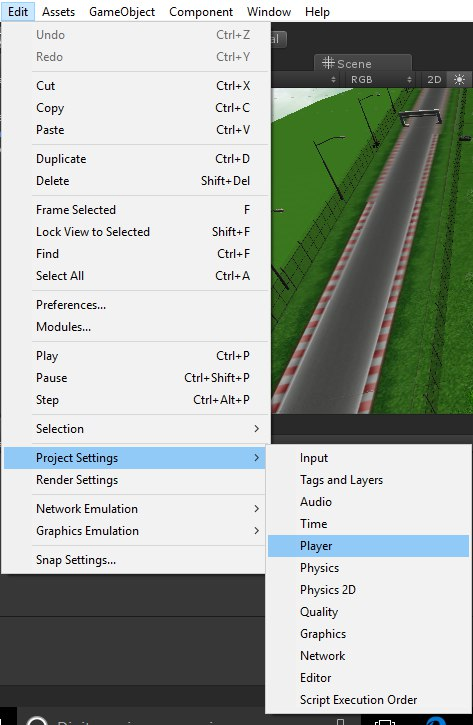
\includegraphics[scale=0.4]{figuras/playersettingspath}
	\captionof{figure}{Caminho para o Player Settings.}
\end{center}

\item Configurar as opções de configuração do Player como o nome do produto, o ícone, o nome da empresa, a resolução padrão do jogo, entre outras.

\begin{center}
	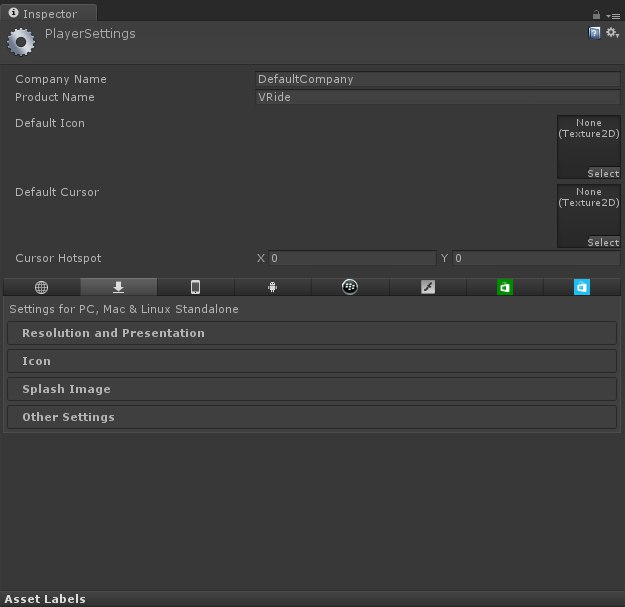
\includegraphics[scale=0.4]{figuras/playersettings}
	\captionof{figure}{Player Settings.}
\end{center}

\item Adicionar todas as cenas no Build Settings. Para isso, é necessário entrar na cena, acessar File > Build Settings e clicar em ``Add current''. As cenas devem ser ordenadas de acordo com o desejado para execução sendo 0 a primeira a ser executada.

\begin{center}
	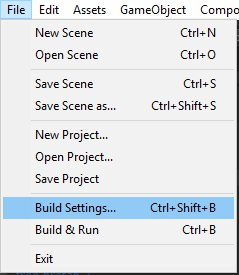
\includegraphics[scale=0.4]{figuras/buildsettingspath}
	\captionof{figure}{Caminho para o Build Settings.}
	\label{fig:buildsettings}
\end{center}

\begin{center}
	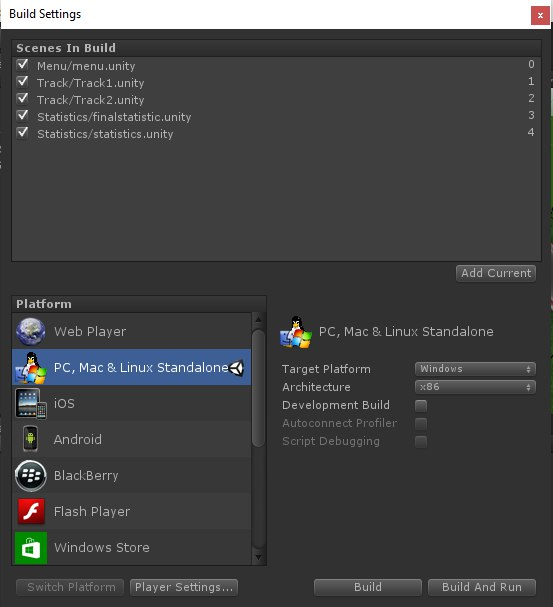
\includegraphics[scale=0.4]{figuras/buildsettings}
	\captionof{figure}{Build Settings.}
	\label{fig:buildsettings}
\end{center}

\item Ainda no Build Settings (Figura \ref{fig:buildsettings}), selecionar a plataforma desejada e apertar em Build.

\item Será carregado o pacote com a extensão desejada.
\end{enumerate}